% !TEX encoding = UTF-8
% !TEX TS-program = pdflatex
% !TEX root = ../Tesi.tex
% !TEX spellcheck = it-IT

%************************************************
\chapter{Modello relazionale}
\label{cap:modello-relazionale}
%************************************************

\section{L'algoritmo di traduzione}
La fase successiva della progettazione di una base di dati consiste nel passare dalla progettazione concettuale alla progettazione logica. Per passare al modello relazionale, si applica un semplice algoritmo.

L'algoritmo che si utilizza per la traduzione dal modello E-R in modello relazionale è formato dalle seguenti operazioni:

\begin{enumerate}
	
	\item
	Traduzione di tipi di entità;
	
	\item
	Traduzione della specializzazione;
	
	\item
	Traduzione di tipi di entità deboli;
	
	\item
	Traduzione di associazioni binarie di tipo $1:1$;
	
	\item
	Traduzione di associazioni binarie di tipo $1:N$;
	
	\item
	Traduzione di associazioni binarie di tipo $N:M$;

\end{enumerate}

\subsection{Traduzione di entità}
	Per ogni tipo di entità (forte) nello schema E-R si costruisce una relazione che contiene tutti gli attributi semplici dell'entità.

\subsection{Traduzione della specializzazione}
	Per ogni tipo di specializzazione dello schema E-R con tipo di entità generale, si costruisce una relazione e si inseriscono tutti gli attributi semplici dell'entità specializzata come attributi della relazione. Si inseriscono come attributi di chiave esterna della relazione gli attributi di chiave primaria delle relazioni corrispondenti ai tipi di entità generali. La chiave primaria della relazione è data dalla combinazione delle chiavi primarie delle entità generali e dalla chiave parziale del tipo di entità specializzata (se esiste).

\subsection{Traduzione di entità deboli}
	Per ogni tipo di entità debole dello schema E-R con tipo di entità proprietario, si costruisce una relazione e si inseriscono tutti gli attributi semplici dell'entità debole come attributi della relazione. Si inseriscono come attributi di chiave esterna della relazione gli attributi di chiave primaria delle relazioni corrispondenti ai tipi di entità proprietari. La chiave primaria della relazione è data dalla combinazione delle chiavi primarie delle entità proprietarie e dalla chiave parziale del tipo di entità debole (se esiste).

\subsection{Traduzione di associazioni binarie 1:1}
	Per ogni tipo di associazione binaria $1:1$ nello schema E-R si individuano le due relazioni coinvolte dall'associazione. Per la traduzione si usa l'approccio basato su chiavi esterne. Si sceglie una delle due relazioni coinvolte, preferibilmente la relazione corrispondente a un tipo di entità con vincolo di partecipazione totale, e si inserisce come chiave esterna la chiave primaria della seconda relazione. Infine si inseriscono sulla relazione scelta tutti gli attributi semplici del tipo di associazione $1:1$.

\subsection{Traduzione di associazioni binarie 1:N}
	Per ogni tipo di associazione binaria $1:N$ nello schema E-R si individuano le due relazioni coinvolte dall'associazione. Per la traduzione si individuata la relazione che rappresenta il tipo di entità partecipante lato-N del tipo di associazione e si inserisce come chiave esterna la chiave primaria della relazione che rappresenta l'altro tipo di entità partecipante all'associazione. Infine si inseriscono sulla relazione scelta tutti gli attributi semplici del tipo di associazione $1:N$.

\subsection{Traduzione di associazioni binarie N:M}
	Per ogni tipo di associazione binaria $M:N$ nello schema E-R si costruisce una nuova relazione che rappresenta l'associazione. Si inseriscono come attributi di chiave esterna della relazione le chiavi primarie delle relazioni che rappresentano i tipi di entità partecipanti, le loro combinazioni formano la chiave primaria della relazione. Infine si inseriscono nella nuova relazione tutti gli attributi semplici del tipo di associazione $M:N$.

\subsection{Traduzione di associazioni ternarie}
	Per ogni tipo di associazione binaria $M:N$ nello schema E-R si costruisce una nuova relazione che rappresenta l'associazione. Si inseriscono come attributi di chiave esterna della relazione le chiavi primarie delle relazioni che rappresentano i tipi di entità partecipanti, le loro combinazioni formano la chiave primaria della relazione. Infine si inseriscono nella nuova relazione tutti gli attributi semplici del tipo di associazione $M:N$.

\section{Applicazione dell'algoritmo di traduzione}
	Di seguito si riporta la traduzione in modello relazionale del modello E-R analizzato:
	
	\begin{figure}[h]
		\centering
		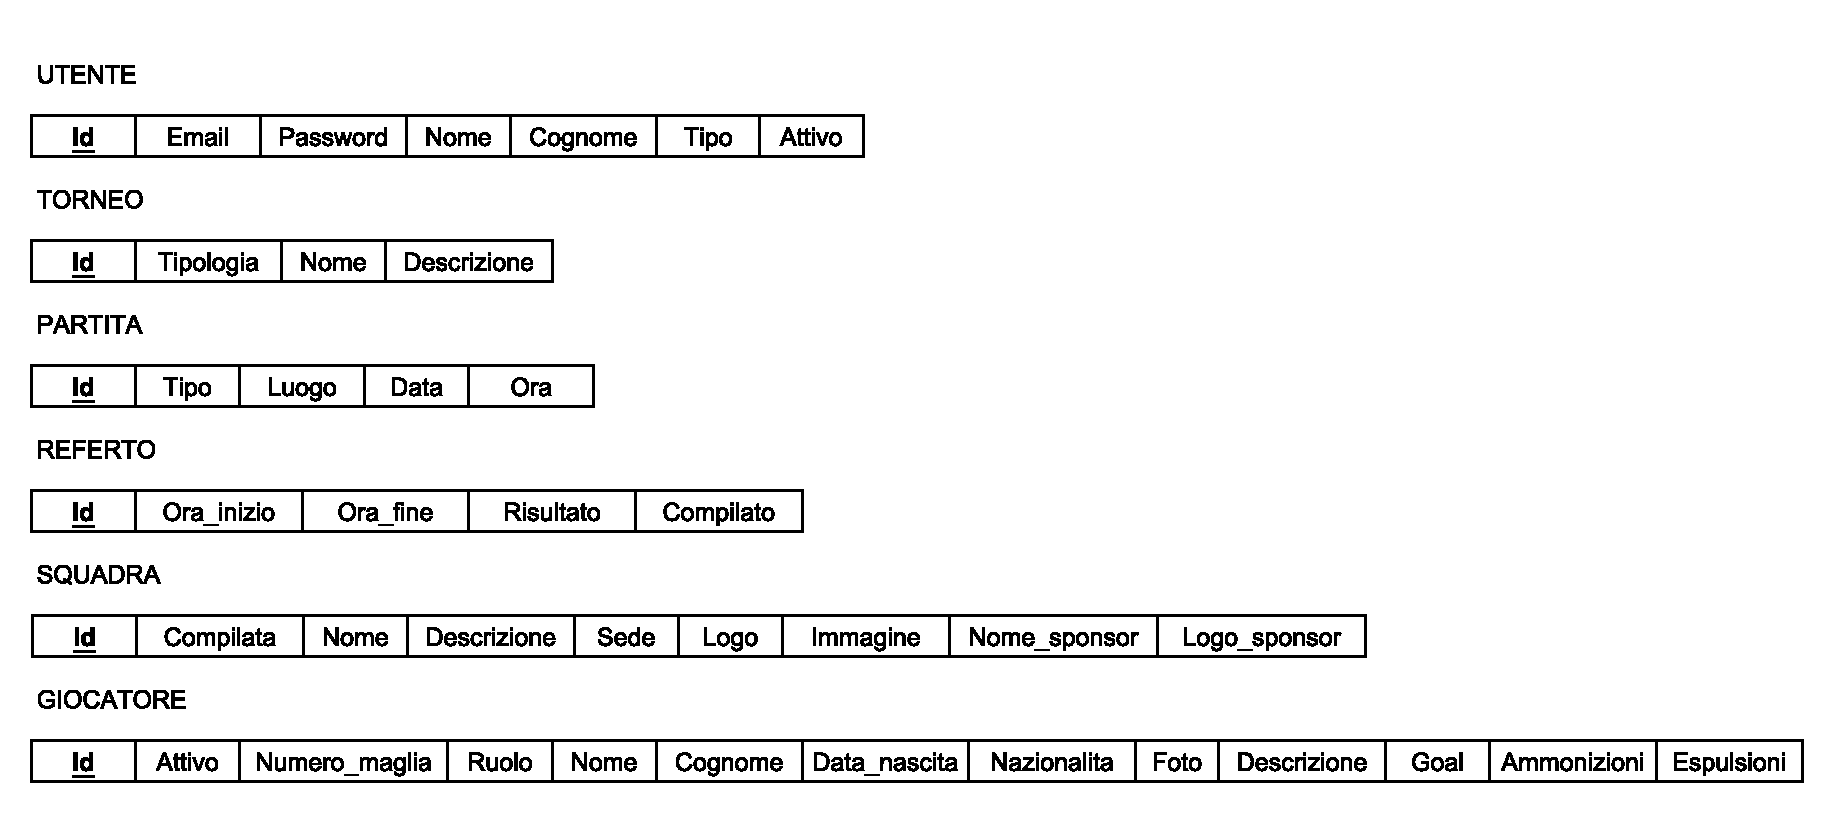
\includegraphics[width=0.85\textwidth]
		{immagini/traduzione-entita}
		
		\caption{Traduzione di entità}
	\end{figure}
	
	\begin{figure}[h]
		\centering
		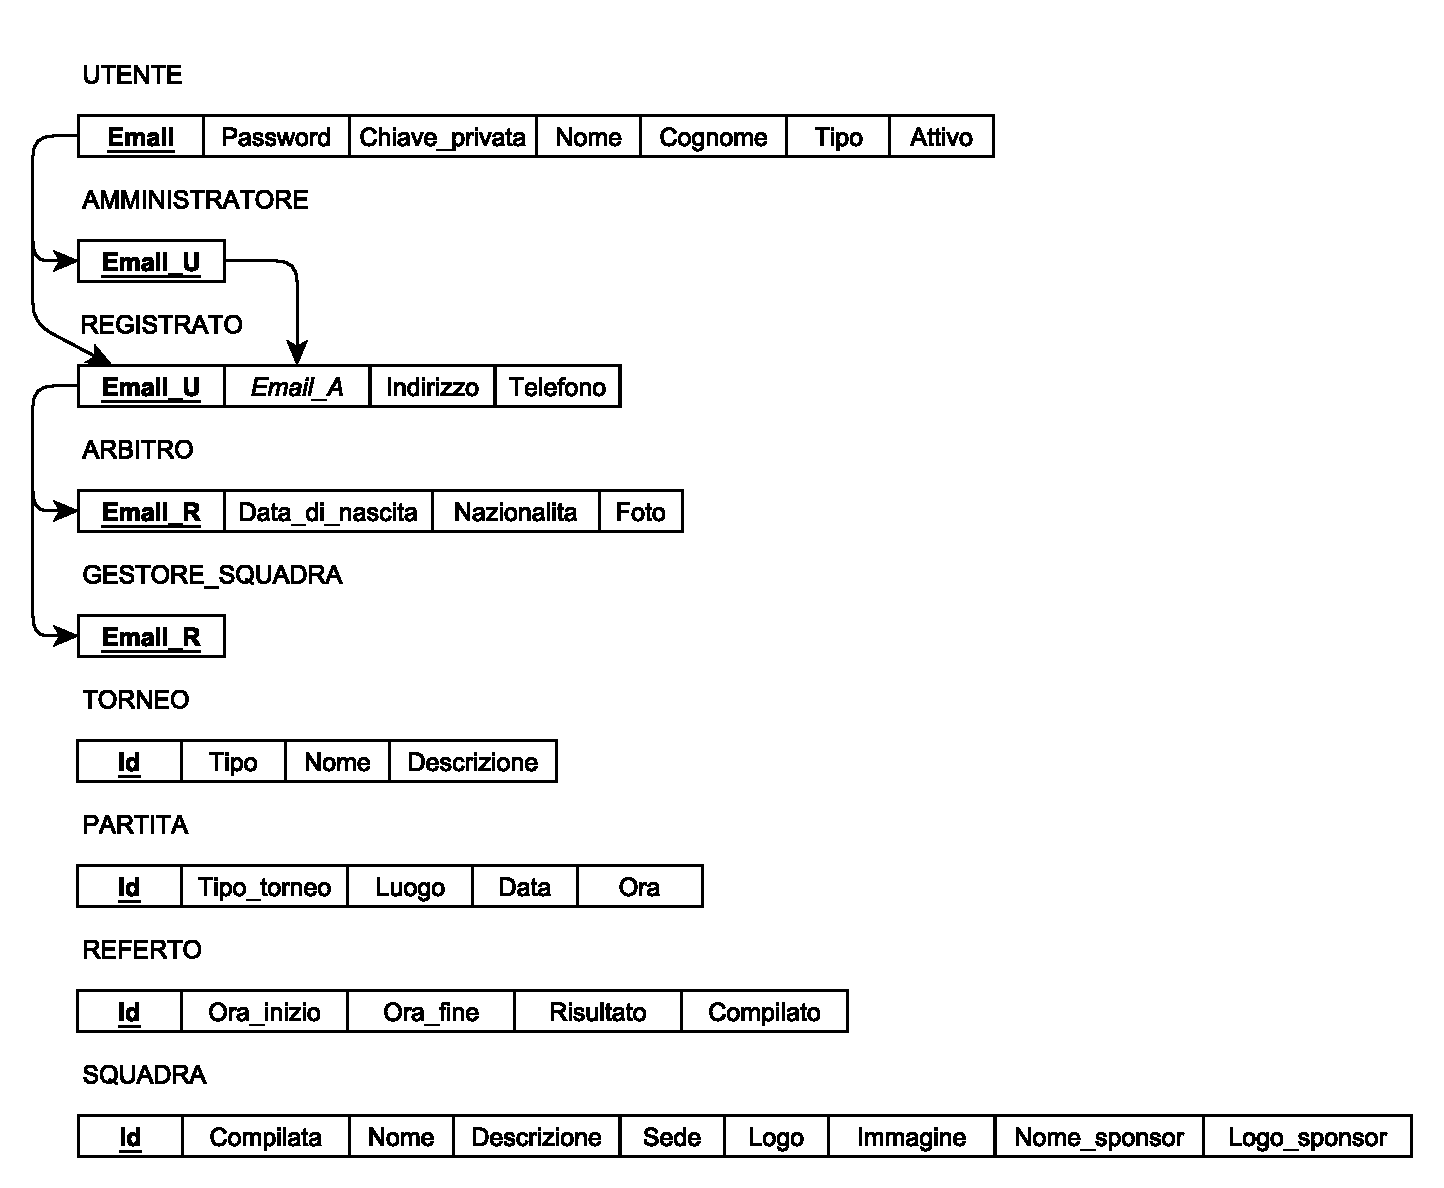
\includegraphics[width=0.95\textwidth]
		{immagini/traduzione-entita-specializzate}
		
		\caption{Traduzione di entità specializzate}
	\end{figure}
	
	\begin{figure}[h]
		\centering
		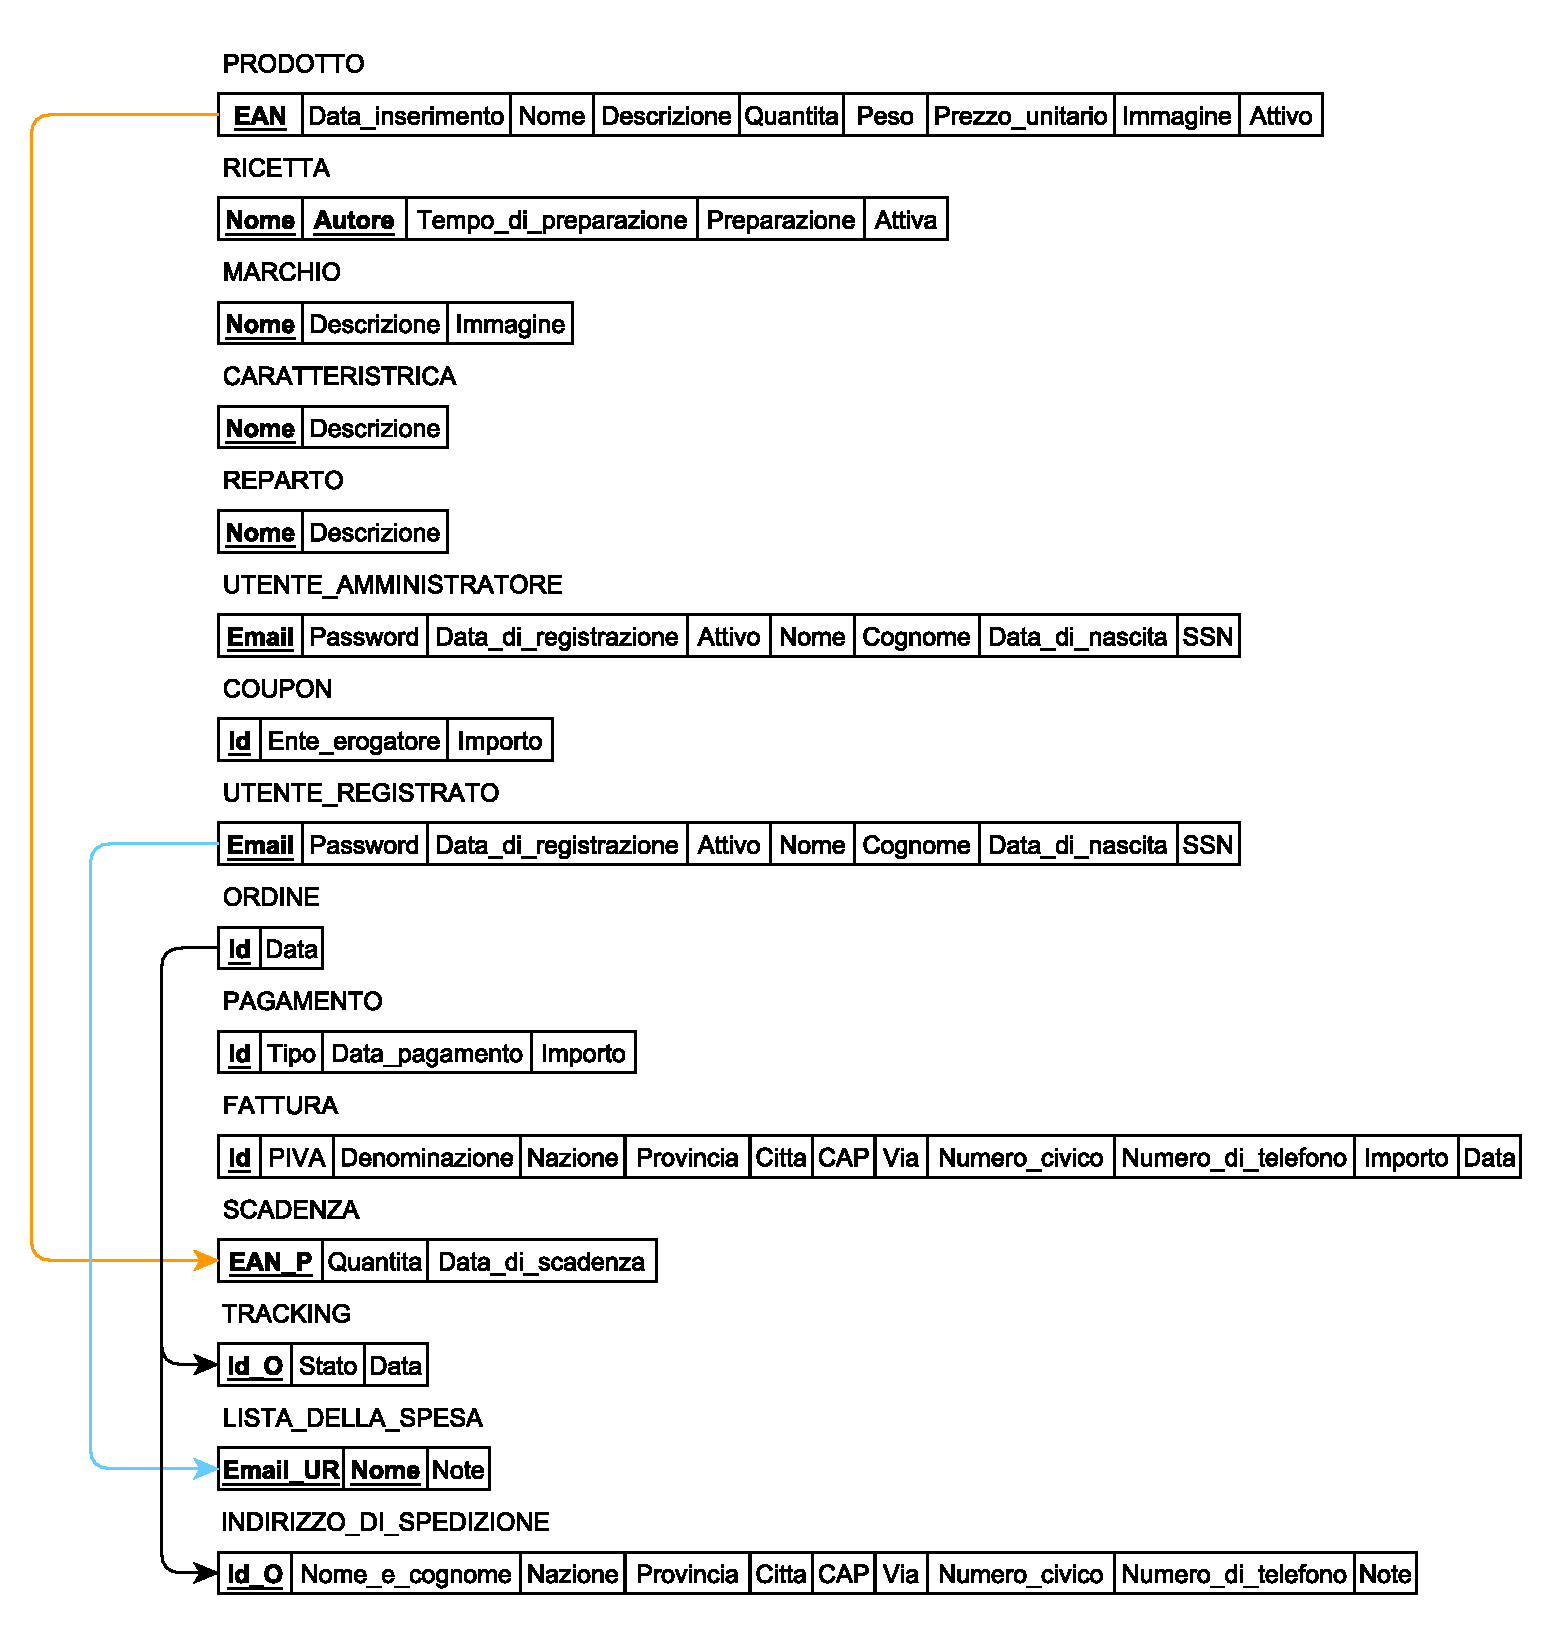
\includegraphics[width=1\textwidth]
		{immagini/traduzione-entita-deboli}
		
		\caption{Traduzione di entità deboli}
	\end{figure}
	
	\begin{figure}[h]
		\centering
		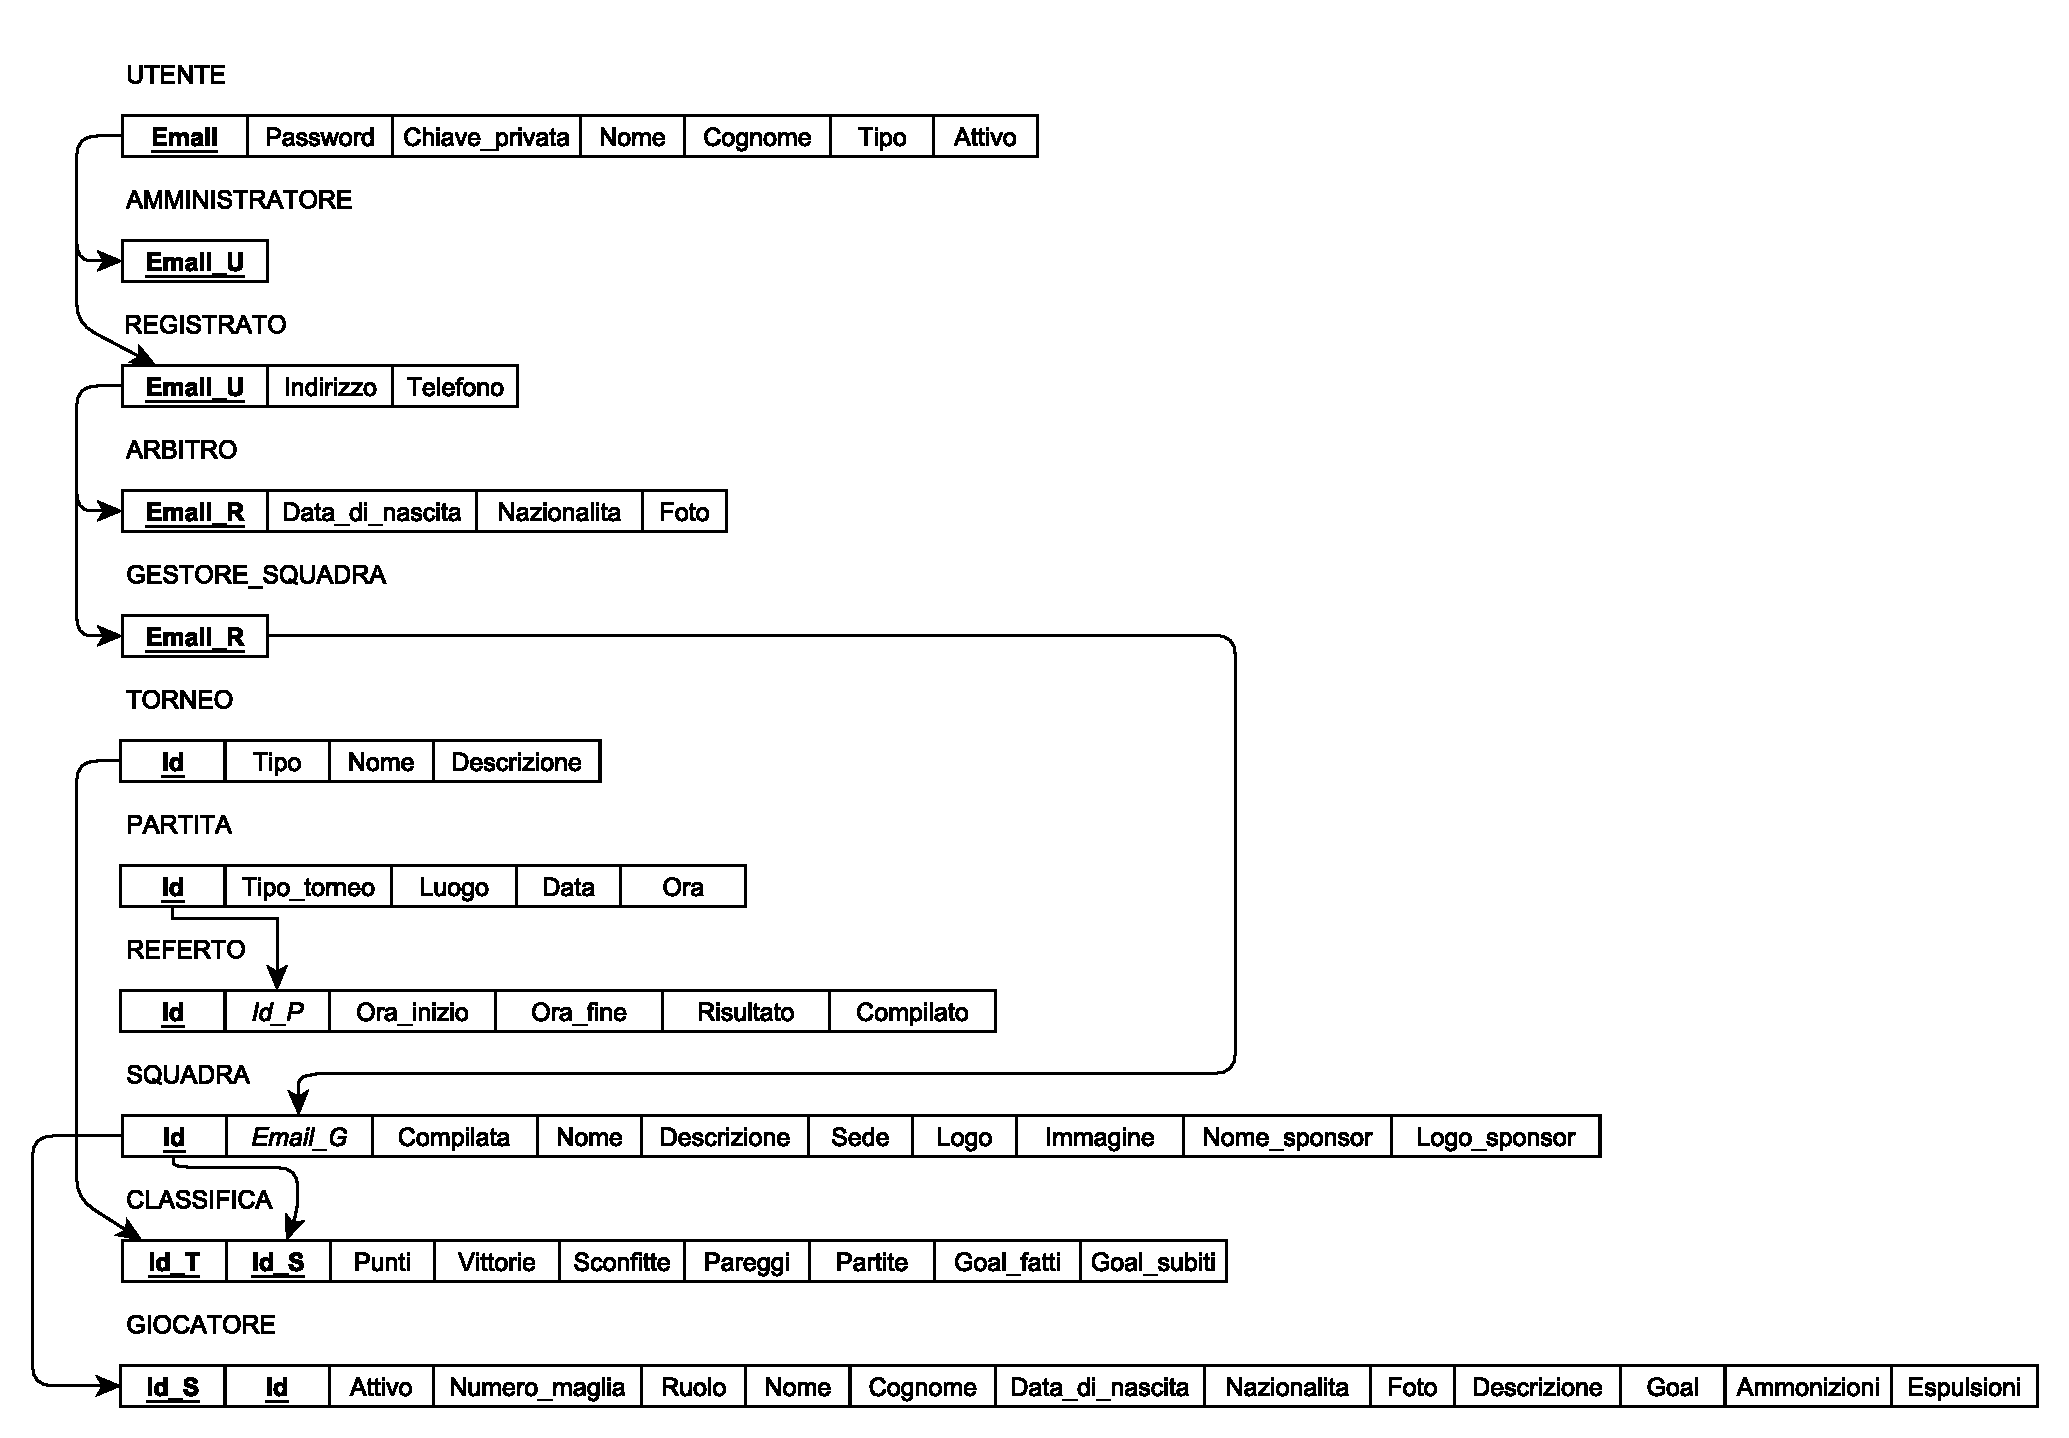
\includegraphics[width=1\textwidth]
		{immagini/traduzione-associazioni-1-1}
		
		\caption{Traduzione di associazioni binarie 1:1}
	\end{figure}
	
	\begin{figure}[h]
		\centering
		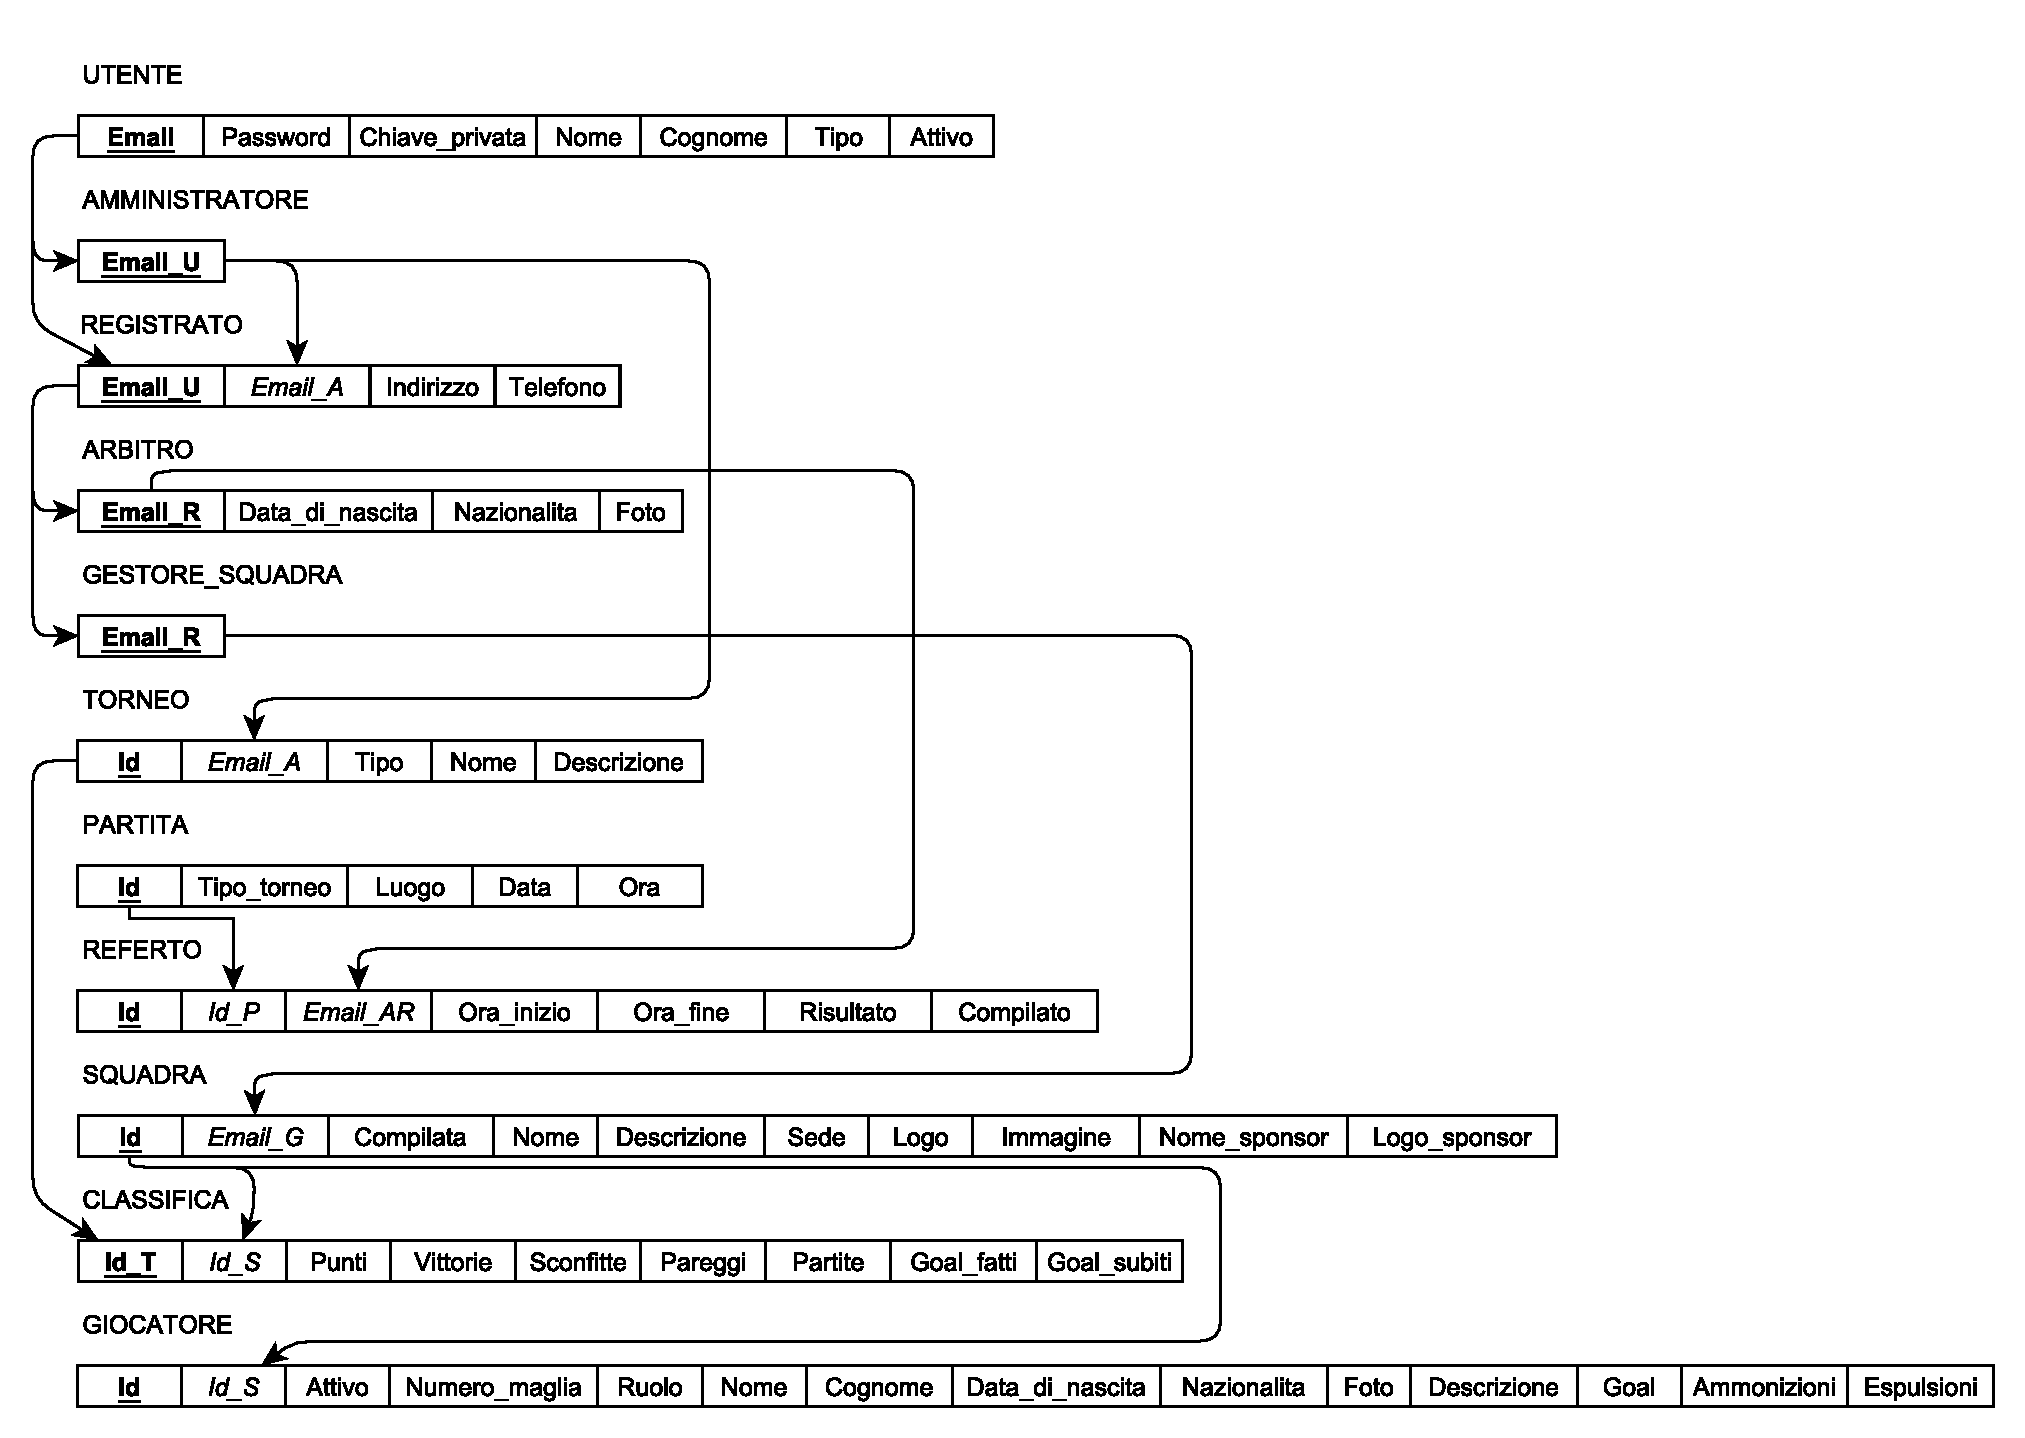
\includegraphics[width=1\textwidth]
		{immagini/traduzione-associazioni-1-N}
		
		\caption{Traduzione di associazioni binarie 1:N}
	\end{figure}
	
	\begin{figure}[h]
		\centering
		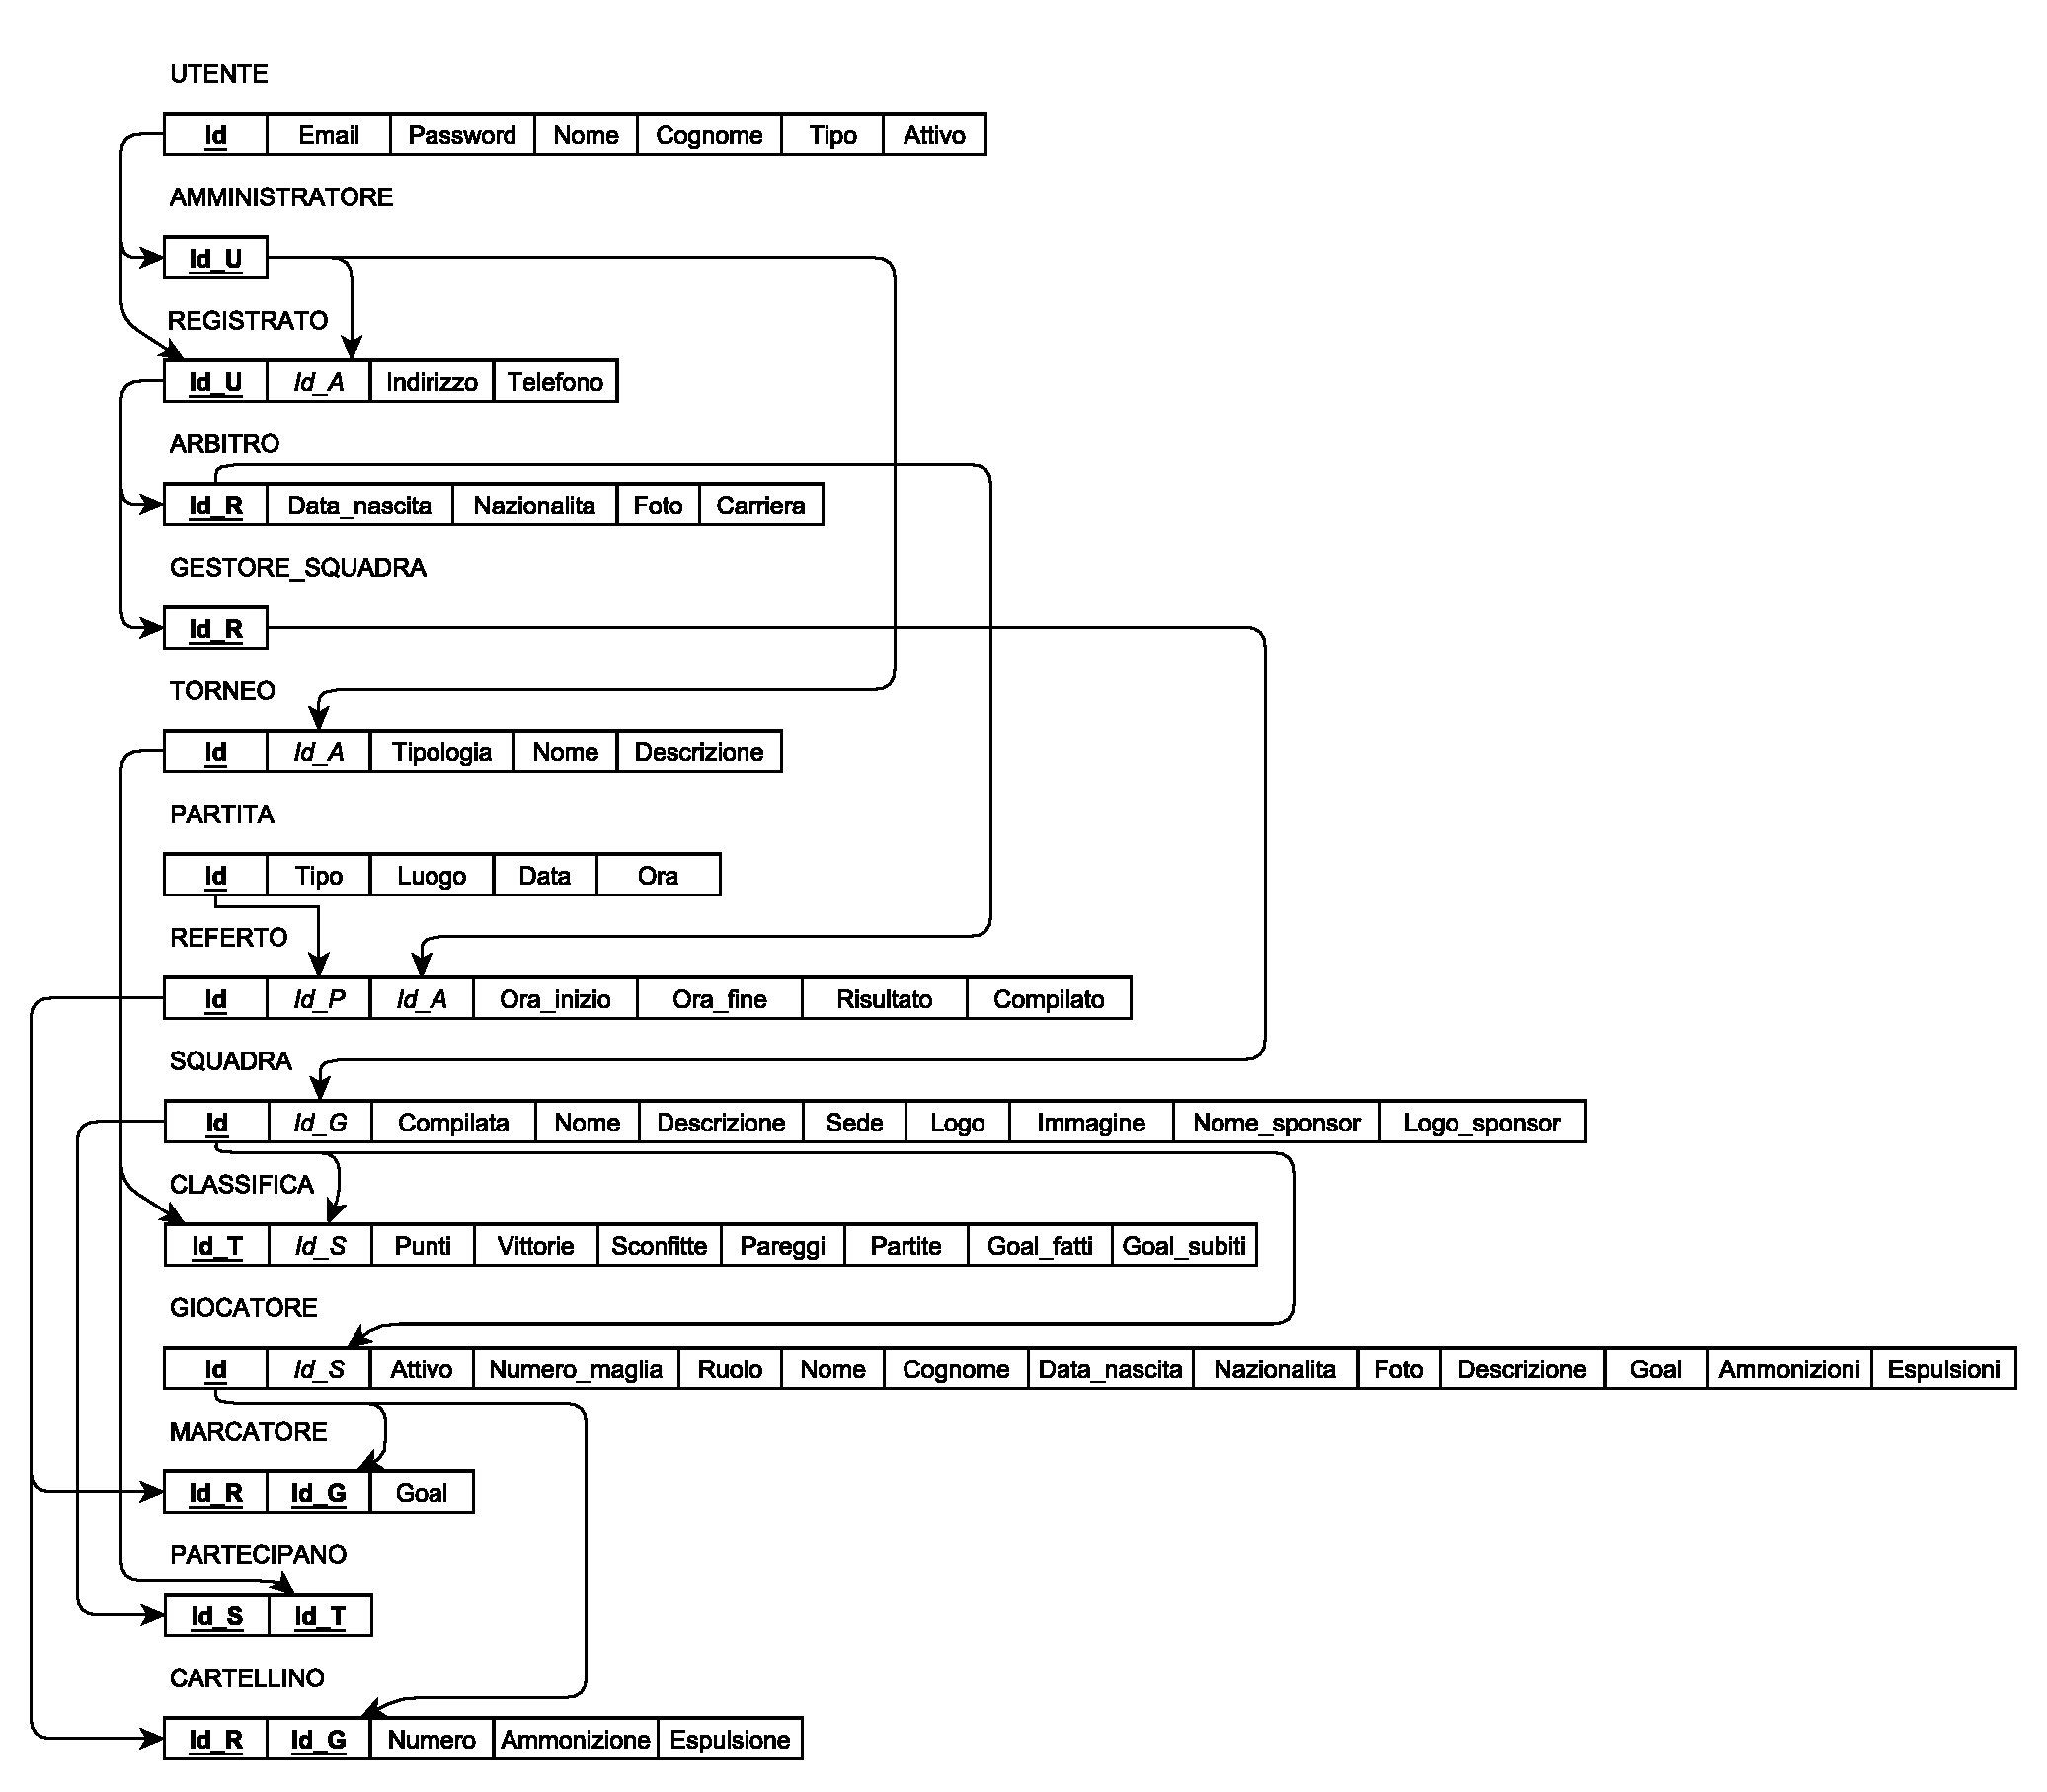
\includegraphics[width=1\textwidth]
		{immagini/traduzione-associazioni-M-N}
		
		\caption{Traduzione di associazioni binarie M:N}
	\end{figure}
	
	\begin{figure}[h]
		\centering
		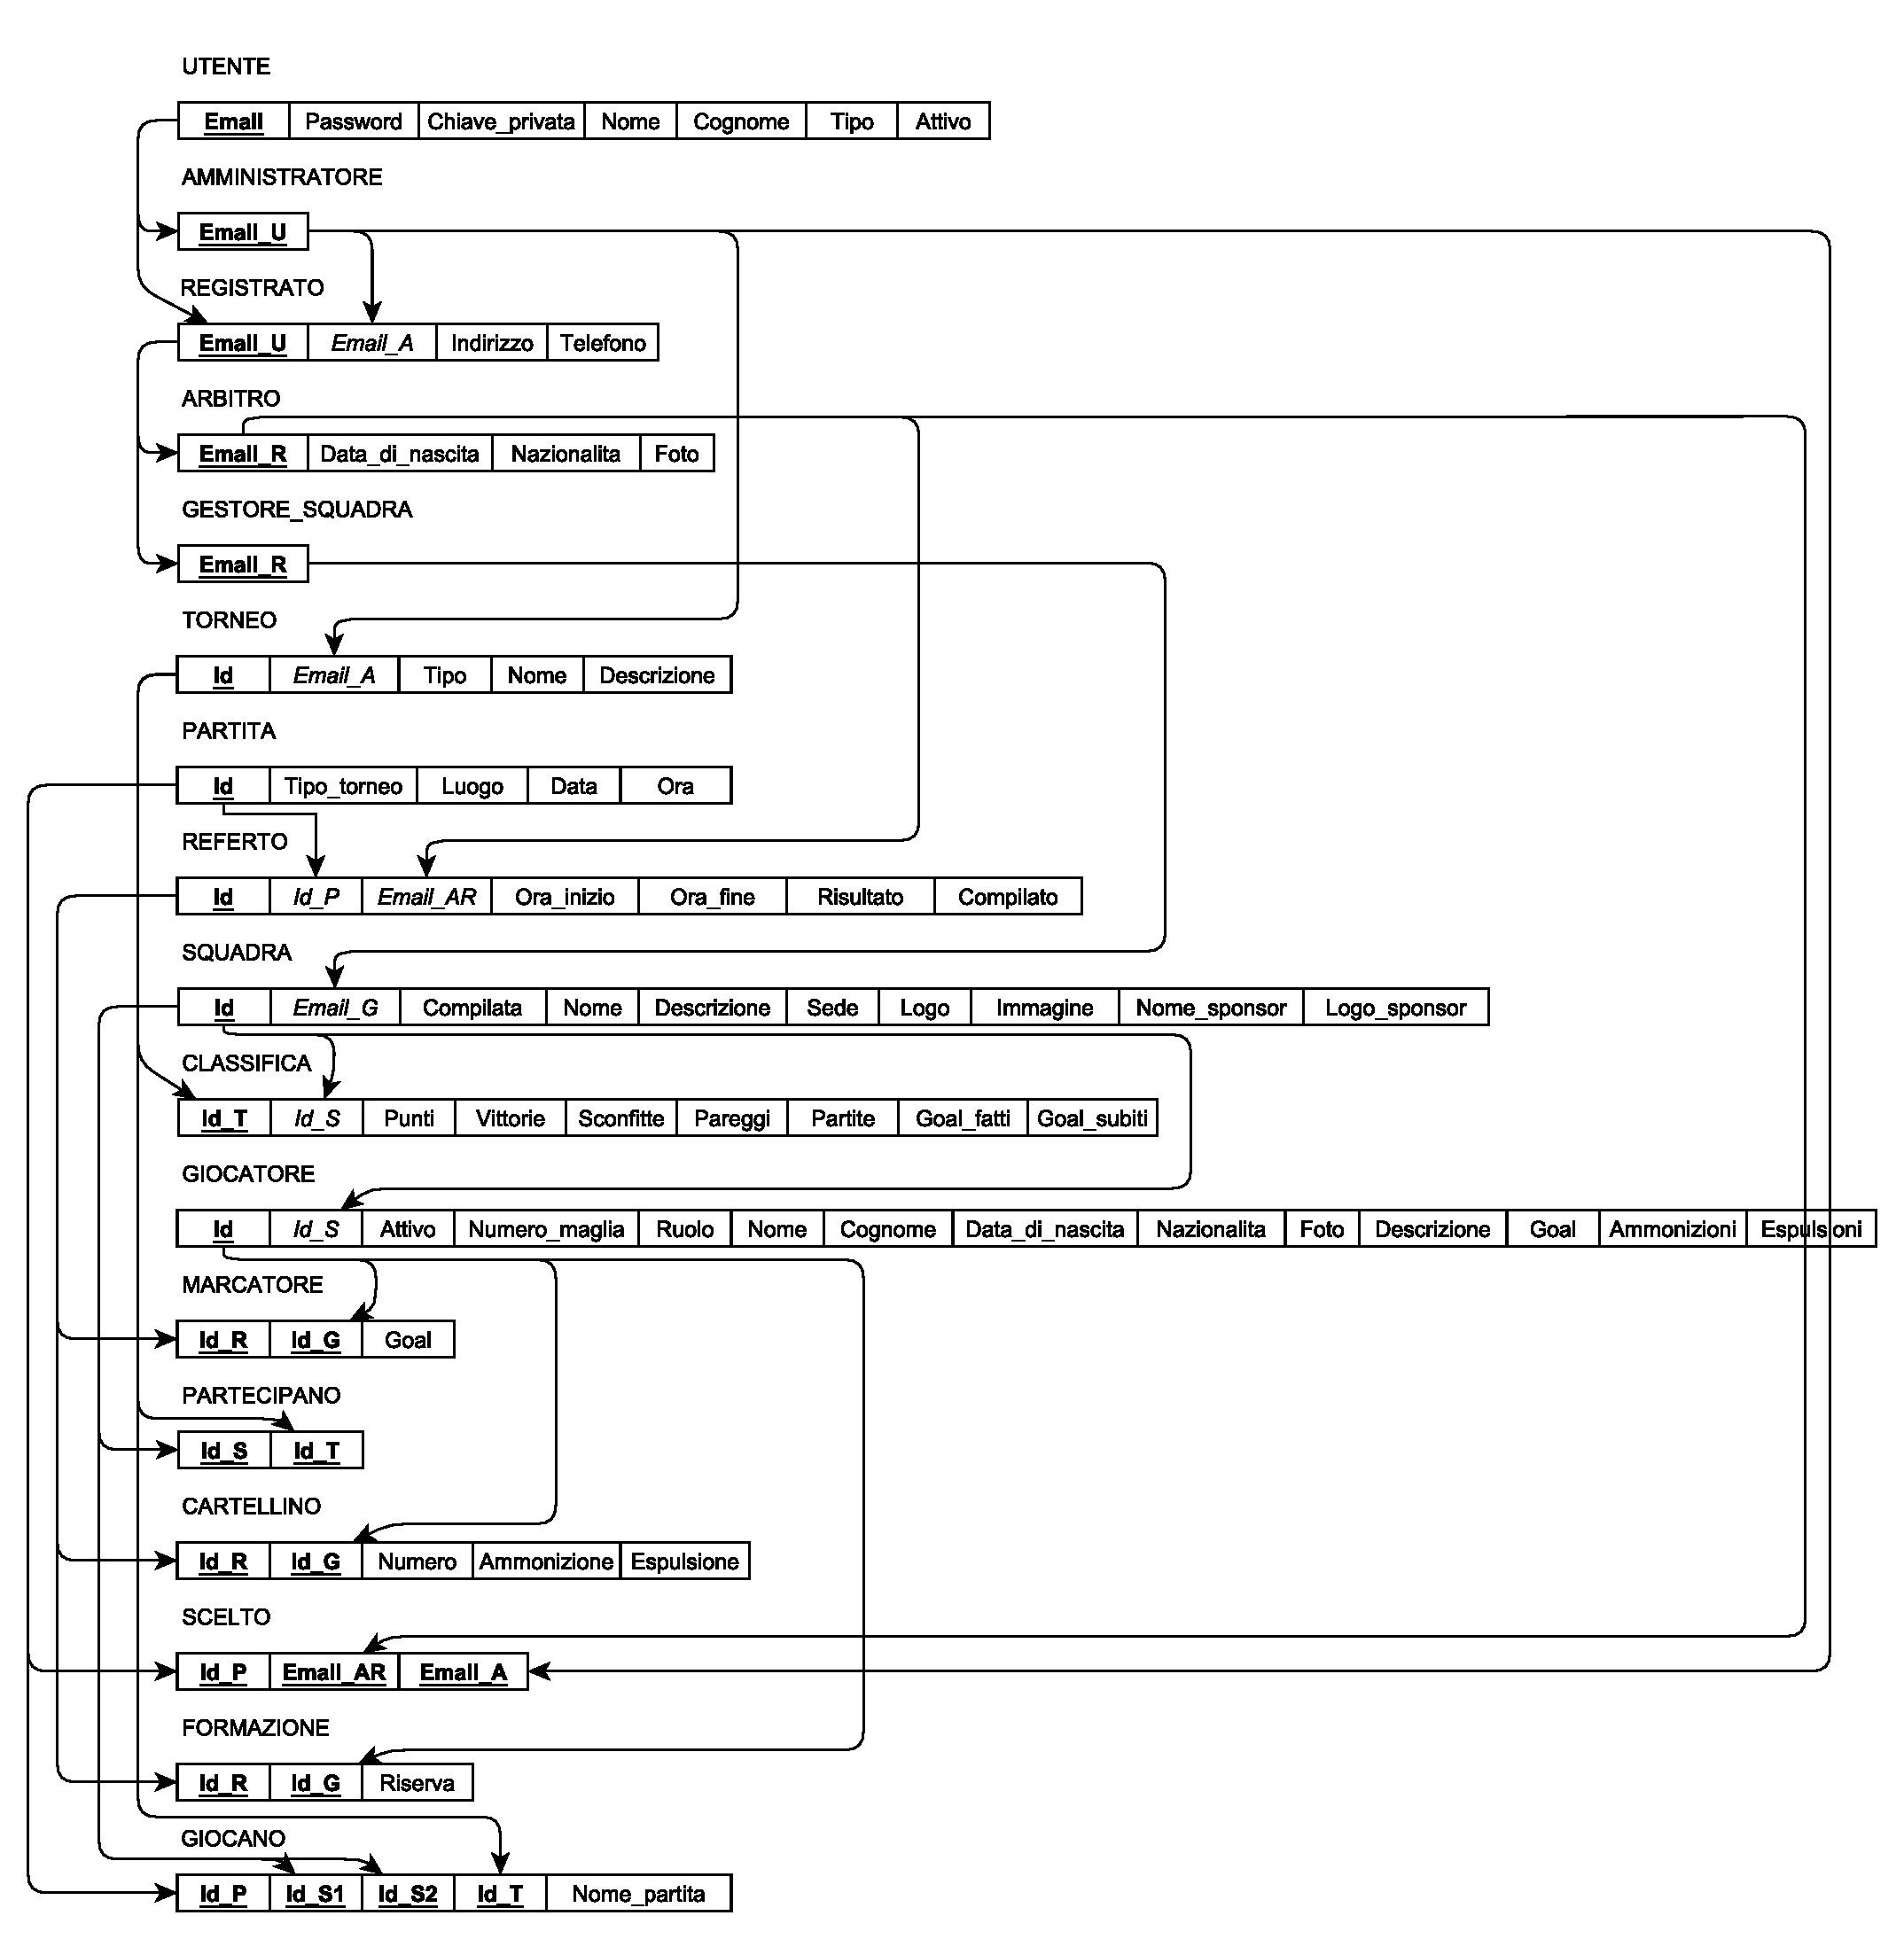
\includegraphics[width=1\textwidth]
		{immagini/traduzione-associazioni-ternarie}
		
		\caption{Traduzione di associazioni ternarie}
		\label{f:trad-assoc}
	\end{figure}